\documentclass{article}
\usepackage{setspace}
\doublespacing
\usepackage[utf8]{inputenc}
\usepackage{amsmath}
\usepackage{fullpage}
\usepackage{enumitem}
\usepackage{graphicx}
\usepackage{grffile}
\usepackage{amsmath}

\usepackage{fancyhdr}
\usepackage{setspace}
\usepackage{titlesec}
\usepackage{caption}
\pagestyle{fancy}

\usepackage{arev}
\usepackage[T1]{fontenc}


\title{Demystifying the Carnegie Classifications: A Sensitivity Analysis}
\author{Paul Harmon\\ Adviser: Dr. Mark Greenwood\\Montana State University}
\date{Spring Semester 2017}
\setlength{\headheight}{20pt}
\renewcommand{\headrulewidth}{0.2pt}
\renewcommand{\footrulewidth}{0.2pt}
\setlength{\parindent}{3pt}
\graphicspath{C:/Users/Paul/Documents/Carnegie Classifications}


\begin{document}
	\maketitle
	\tableofcontents



\subsection{other crap}
\begin{figure}
	\includegraphics[.8\textwidth](C:/Users/Paul/Documents/Carnegie Classifications/"mbc3".png)
	\caption{\label{fig:mbc2} The model-based cluster solution is given below with the optimal number of clusters.}
\end{figure}

 \begin{figure}
	\centering
	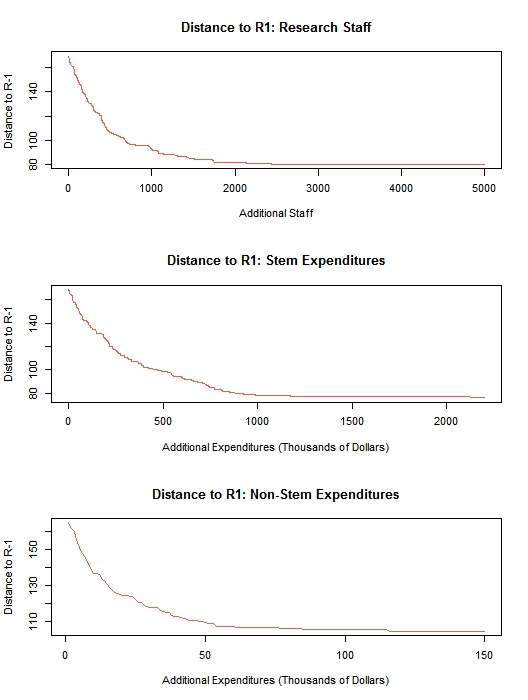
\includegraphics[width=.7\textwidth]{C:/Users/Paul/Documents/Carnegie Classifications/DistR1both}
	\captionsetup{font=footnotesize,labelfont=footnotesize}
	\caption{\label{fig:agb} }{Single Variable Movement: Changes in expenditures and research staff lead to movement in all directions since they are used in both indices. However, increases in any single variable do not lead to large enough movement to get across the R1 threshold.}
	
\end{figure}


\subsubsection{Similar R2 Institutions}
Examining the classifications allows for administrators and other decision makers at Montana State to identify a cohort of similar institutions; that is, after all, the purpose for which the classifications are designed. It is possible to get a sense for the nearest neighbors to Montana State. Figure 1 shows the plot of the most similar institutions to Montana State. 

It is evident that University of Alaska-Fairbanks is the institution that most closely resembles Montana State. Interestingly enough, when comparing the raw numbers, they do not look all that similar; Montana State is clearly more productive in producing doctorates in every category save for Social Sciences. Further, while Alaska-Fairbanks spends more money on STEM expenditures, Montana State spends more on non-STEM and has a larger research staff cohort.  The key similarities lie not in the raw data but the averaged rankings. Table \ref{tab:UAA} gives the actual values of each variable for the two schools.

Institutional researchers ought to use this cohort of nearest neighbor schools to make meaningful comparisons. From a research perspective, for instance, Carnegie Mellon University, Oregon State University, and Rice University are more similar to Montana State in terms of research characteristics than they are to the large-scale R1 schools such as Stanford, Johns Hopkins or the University of Washington. The cohort of similar institutions is given in Table \ref{tab:nn}.


% latex table generated in R 3.3.2 by xtable 1.8-2 package
% Sun Apr 23 09:37:44 2017
\begin{table}[h]
\centering
\begin{tabular}{|rrrrrrrrr|}
  \hline
NAME & FACULTY & HUM & OTHER & SOSC & STEM & STAFF & STEM Exp & NS Exp \\ 
  \hline
Montana State &   456 &   2 &   9 &   0 &  45 &  75 & 104646 & 8702 \\ 
Alaska Fairbanks &   374 &   1 &   5 &   4 &  34 &  50 & 152352 & 3417 \\ 
   \hline
\end{tabular}
\caption{\label{tab:UAA} Comparison of Montana State to University of Alaska Fairbanks. Although not similar across all values on the raw data, both universities have similar scores on the Carnegie indices. }
\end{table}




% latex table generated in R 3.3.2 by xtable 1.8-2 package
% Sun Apr 23 09:48:19 2017
\begin{table}[ht]
\centering
\begin{tabular}{|lll|}
  \hline
 ID Number & Name & Distance from MSU \\ 
  \hline
6 & University of Alaska Fairbanks & 0.02 \\ 
146 & Dartmouth College & 0.12 \\ 
177 & Yeshiva University & 0.24 \\ 
 165 & Rensselaer Polytechnic Institute & 0.28 \\ 
 34 & Colorado School of Mines & 0.36 \\ 
 24 & Naval Postgraduate School & 0.39 \\ 
 168 & Rockefeller University & 0.42 \\ 
  187 & North Dakota State University-Main Campus & 0.36 \\ 
  147 & University of New Hampshire-Main Campus & 0.44 \\ 
  118 & Tufts University & 0.56 \\ 
  204 & Oregon State University & 0.58 \\ 
  99 & Tulane University of Louisiana & 0.67 \\ 
  238 & Rice University & 0.67 \\ 
  207 & Carnegie Mellon University & 0.74 \\ 
  246 & The University of Texas at Dallas & 0.66 \\ 
   \hline
\end{tabular}
\caption{\label{tab:nn} Comparison of Montana State to nearest neighbors. Montana State's cohort of similar schools includes an impressive cohort of institutions, both R1 and R2. Distances are scaled Euclidean distances from Montana State. }
\end{table}

\subsubsection{Montana State compared to R1 Institutions}

In 2010, Montana State was classified as an R1 institution. The reason for this is not entirely clear; however, Montana State had a high per-capita index value and continued to have this in 2015; the per-capita score for Montana State was above the 75th percentile.  

Of all doctoral-granting institutions, Montana State's research expenditures on STEM-related fields were above the median value, as were its non-STEM expenditures. That, combined with the above-median research staff size, may explain why the Montana State scored highly on the per-capita scale. However, output in terms of PhD degrees awarded is less than the 50th percentile for all degree types awarded, even STEM doctorates. A naive look at the data makes it appear that Montana State would be reasonably well-classified in the R1 group. As seen in Table \ref{tab:r1}, outside of Social Science PhDs, MSU produces PhDs, spends research money, and hires research staff at a rate that would be relatively similar to many of the smaller R1 schools. 



% latex table generated in R 3.3.2 by xtable 1.8-2 package
% Sat Apr 22 21:34:02 2017
\begin{table}[ht]
\centering
\begin{tabular}{|rrrrrrrr|}
  \hline
 & HUM & OTHER & SOSC & STEM & Staff & Stem & NonStem \\ 
  \hline
Montana State University & 2.00 & 9.00 & 0.00 & 45.00 & 75.00 & 104646.00 & 8702.00 \\ 
  Mean R1 & 51.00 & 87.00 & 44.00 & 202.00 & 604.00 & 411742.00 & 21672.00 \\ 
  Median R1 & 45.00 & 76.00 & 37.00 & 152.00 & 387.00 & 319818.00 & 14914.00 \\ 
  Min R1 & 0.00 & 0.00 & 1.00 & 27.00 & 32.00 & 5719.00 & 725.00 \\ 
   \hline
\end{tabular}
\caption{\label{tab:r1} Comparison of Montana State to R1 schools. MSU looks like it could fit in on any single metric, but would be near the bottom when considering all variables. }
\end{table}

Many R2 schools have instituted policy goals geared towards moving from the "lesser" R2 category to the R1 category. Indeed, both the University of Idaho (McClintick 2016) and the University of Montana (University of Montana 2017) are making R1 a policy goal. But is this a reasonable goal for Montana State? Does Montana State compare favorably with R1 schools on the metrics used to calculate the Carnegie Classifications? 

However, comparing MSU on each metric to R1 schools is misleading. It is worth recalling that the Carnegie Classifications are based on weighted averages of these covariates, not the individual variables themselves. Thus, a more fair comparison would be to look at Montana State across all metrics vs. R1 schools on all metrics. This can be achieved with a Parallel Coordinate Plot, as is given in Figure \ref{fig:matplot}. The nearest R1 schools, Oregon State and Tufts Universities, are both shown as well. The difference between the majority of R1 schools and Montana State is striking; MSU produces fewer PhDs across the board and spends less money on research than nearly all of the schools in the top tier category. Even if Montana State were classified in the R1 group, it would be near the minimum in all categories. In 2015, Montana State lagged behind most of the R1 institutions in expenditures, staff sizes, and doctorates awarded. While Montana State had more Other, Humanities, and Stem doctorates awarded than the smallest R1 institutions, it lagged behind the mean and median R1 values by a large margin. Moreover, expenditures and research staff sizes were much smaller than the average R1 schools, even if they were slightly larger than the smallest R1 school.






\section{Principal Components Analysis}
\subsection{What is PCA}
The Carnegie Classifications are built using a methodology known as Principal Components Analysis (PCA). The main goal of PCA is to do dimension reduction. Often, it is of interest to take a large set of variables and reduce it down to a more manageable number of covariates. Consider a set of p predictors $x_1, x_2,...x_p$. Methods for dimension reduction such as Principal Components Analysis seek to reduce the number of $p$ covariates by creating a new set of covariates $y_1, y_2,...y_q$ via an eigenvalue decomposition of either the correlation matrix or covariance matrix of the X's. These $y$ variables are then interpreted as functions of the x's; further, they are ordered so that the first new variable, $y_1$, accounts for the most variation in the original $x$ covariates (Everitt and Hothorn 2011). Note that we have not yet achieved dimension reduction; PCA by itself returns the same number of re parameterized covariates as what we started with. However, since the new covariates contain information about the variation in the old covariates, it is possible to use only a subset of the first few $y$ variables without losing much information about the variation in the $x$'s.  In this way, often the first two or three $y$'s are used to describe the entire set of q $x$'s.

\subsection{Calculating Scores and  Loadings}
Principal components analysis returns two key pieces of information: the \textbf{scores} and the \textbf{loadings}. In the more general case of factor analysis, of which PCA is just a single method, the scores are sometimes referred to as factors. The scores are the aforementioned $y$ values.  

The first principal component, $y_1$ can be represented as follows for the $x_{1},...,x_{q}$ original covariates:
$y_1 = a_{11}x_{1} + a_{12}x_{12} + ... + a_{1q}x_{q}$ 

The scores can be thought of as an "index" for a more complicated underlying process; each score is a weighted average of the original $x$ variables. In the Carnegie Classifications, the researchers explicitly define the scores used in the analysis as a "per-capita index" and an "aggregate index."  

The loadings, then, are the coefficients by which each original covariate must be multiplied obtain the original data. These are standardized by dividing by the square root of the eigenvalues themselves. The scores can be interpreted as weighted averages of the original covariates; the loadings are the weights on which those averages are calculated. 

PCA can be done on either the correlation matrix, or the covariance matrix(Everitt and Hothorn 2011). In the Carnegie Classifications, the correlation matrices were used. In R, calculation of the Principal Components Analysis can be done using the function \texttt {prcomp} (R Core Team, 2017).  

\subsection{Dimension Reduction: How Many Scores Should Be Used}
The question of how many scores should be used has no definitive answer; it is often left up to the researcher to define the optimal degree of dimension reduction. Certainly, the number of scores used should be less than the original number of covariates; otherwise, the researcher might as well work with the original data. 

In the Carnegie Classifications, the researchers used only the first score for each index created. This allowed for researchers to directly plot two independently-calculated indices against each other; however, using only a single score for the index means that they explained less variance in the original covariates. Indeed, in the 2015 update the aggregate index score only explained 70 percent of the variation in the original data and the per-capita index explained only 71 percent (Borden 2017).  


\subsection{Regression and Classification}
Principal Components Analysis is a powerful tool for dimension reduction; it can be used both in a classification setting and a regression setting. For classification, using the singular value decomposition to create a subset of k principal components scores allows for comparison on a reduced set of covariates. In regression, the linear predictor can be rewritten as $y = \textbf{X} \beta + \epsilon = \textbf{F}\theta + \epsilon$ where \textbf{F} is called the Factor Matrix; it contains only the set of k scores (West 2003). Singular Value Regression, or Principal Components Regression, is useful for some regression problems.  This analysis focuses mainly on the classification aspect of PCA; however, it is worth noting that the methods used here could be utilized in a regression setting for prediction. As pointed out by Everitt and Hothorn, PCA is "overwhelmingly an exploratory technique"(Everitt and Hothorn 63) and in the case of the Carnegie Classifications, it is used largely to describe graphically the differences between institutions rather than to predict them. 
\pagebreak
\section{Recreating The Carnegie Classifications}
\subsection{The 2015 Update}
The classifications are calculated from two different indices, one on the aggregate counts for each institution, and the other on a per-capita basis. The classifications themselves do not count the per-capita measures based on student populations at each school; rather, they focus on the size of the faculty at each institution in terms of a raw headcount of tenurable and non-tenurable faculty.\\
In general, institutions with relatively large values in one index are likely to be relatively large in the other index. In 2010 the correlation between the two indices was a strong positive 0.83. In 2015 the correlation was 0.84.  The two indices are calculated in the following way: 
\begin{enumerate}
\item Each variable is ranked from smallest to largest. Ties are all assigned the minimum rank.
\item Two Principal Components Analyses are fit on the ranked data.
\item An Aggregate and Per-Capita Index are calculated from the first Principal Component of each PCA.
\item The indices are rescaled and new Aggregate Index is plotted against the new Per-Capita Index to create Figure 1.
\item Arcs are drawn with arbitrary radii to define breakpoints between categories.
\end{enumerate}

\subsection{Why Rank the Data?}
There is no mathematical reason that the indices could not be based on the raw counts of PhDs, research staff, and expenditures. However, large schools tend to produce research and spend money at much higher rates than smaller schools.  Counts of PhDs awarded, expenditures, and research staff/faculty sizes are therefore severely positively skewed. For instance, Johns Hopkins spent over 2 billion dollars on STEM expenditures in 2015 - Montana State spent only 104 million dollars by comparison.   Ranking the data prior to classification increases separation between institutions at the low end and decreases separation between institutions with large variable values. Figure \ref{fig:beanplots} shows beanplots (Kampstra 2008) that display the distributions of both the ranked and raw data. The narrow lines refer to each institution's value in the dataset; the wide lines refer to the mean values for each variable.  \\



\subsection{Aggregate Index}
 The aggregate index includes PhD degrees awarded in humanities, professional fields, social sciences, and stem fields; however, it also includes the research staff, stem expenditures, and non-stem expenditures from the Per Capita Calculation.\\
 The formula for the aggregate index is given below for the ith institution:
 \begin{center}
	\begin{equation}
	\centering
	$$AggregateIndex_{i} =  .37HumD^{*}_{i} + .27StemD^{*}_{i} + .39SocSciD^{*}_{i} + .27OtherD^{*}_{i} $$
	$$ + .40StemExp^{*}_{i} + .38NonStem^{*}_{i} + .33ResStaff^{*}_{i} $$
	\label{eqn:agindex}

	\end{equation}
\end{center}

  \subsection{Per Capita Index}
 The per-capita index considers only three variables: non-faculty research staff, stem expenditures, and non-stem research expenditures divided by the size of the faculty at the given institution. The weights on each variable are calculated from the loadings generated by the per-capita PCA. \\
     The formula for the per-capita index is given below for the ith institution:
     
     \begin{equation}
     \centering
     PerCapitaIndex_{i} = \frac{.64ResStaff^*_{i} + .64StemExp^*_{i} + .42NonStemExp^*_{i}}{FacultySize^*_{i}}
     \label{eqn:Per Capita Index}
     \end{equation}
     
   
  \subsection{Combining the Indices}
  After calculating the individual per-capita and aggregate indices, the two are combined with a single plot. The per capita ranking is plotted along the X axis and the aggregate ranking is plotted along the y-axis. The Carnegie Classifications are then based on the natural spacing that occurs in the data; in some years the data are fairly well separated into three clusters and in other years they are not. \\
  In 2015, no obvious clusters were formed; further, there were no obvious spaces of separation that would define the two borders between the three groups. The classifications were found by dividing the per-capita index roughly into three groups and finding the areas of greatest separation between points in that region. In the 2010 update, the lines that divided groups were hand drawn; however, in 2010 the lines were drawn by calculating circles with uniform radius from the origin. Using circles allows for institutions with outlying scores in a single index to be more likely to end up in the highest classification. 
  \subsection{Method For Ties}
 In replicating the classification done by the Carnegie Institute, only a handful of decisions must be made. The most important choice comes in the ranking step. When ranking institutions that are tied, there are several methods for calculating rank that have important consequences for an analysis, especially where an institution can move up or down in rank in subsequent years. In the statistical software package R (R Core Team), the default setting of the rank function is to take the average of the ranks (Becker et. al. 1988). For instance, if the first five institutions have the same value for Stem Expenditures, each institution would receive a rank value of 2.5.  Alternative methods include taking the first, last, minimum, or maximum of the ranks.  The first and last methods result in taking a permutation of each of the potential ranks with first involving increasing values and last involving decreasing values. The minimum rank method refers to the more commonly known ranking method used in sports; in the previous example, each of the five institutions would be ranked 1st. Similarly, the maximum rank gives the largest rank to all of the observations; in the previous example, each institution would be ranked fifth. \\
The literature on the Carnegie Classifications does not specify exactly the method that the institute used for tied ranks, but comparing each method to the final results indicates a clear picture. Below is a table of standardized loadings for each method along with the loadings generated from the actual classifications. 

\begin{table}[h]
\centering
\begin{tabular}{rrrrrrrr}
	\hline
\textbf{Aggregate Rankings}\\
\hline
Ties Method & HUM &OTHER&SOSC&  STEM & STAFF & STEM exp & NS exp \\
Average     &0.83	&0.618	&0.881	&0.916  &0.907	&0.899	&0.792\\
First       &0.822	&0.615	&0.882	&0.918	&0.908	&0.899	&0.788\\
Last        &0.824	&0.62	&0.876	&0.913	&0.907	&0.899	&0.795\\
Min         &0.818	&0.616	&0.873	&0.914	&0.902	&0.899	&0.792\\
Max         &0.837	&0.619	&0.886	&0.917	&0.912	&0.899	&0.792\\
Actual      &0.82	&0.617	&0.874	&0.915	&0.902	&0.9	&0.79\\
\hline
\textbf{Per Capita Rankings}\\
\hline
Average&-&-	&-	&-  &0.93	&0.932	&0.615\\
First&-&-	&-	&-  &0.93	&0.933	&0.61\\
Last&-&-	&-	&- &0.929	&0.932	&0.615\\
Min&-&-	&-	&-  &0.928	&0.93	&0.616\\
Max&-&-	&-	&-  &0.93	&0.934	&0.615\\
Actual&-&-	&-	&-  &0.928	&0.931	&0.614\\
\hline

\end{tabular}
\caption{\label{tab:ties} Standardized Loadings: The standardized loadings generated with the minimum method for ties had the most exact matches and the closest overall matches to the actual Carnegie Classifications. The small differences may be due to software or rounding differences. }
\end{table}

Moreover, the plots generated by each of the methods confirm that the minimum ranking was used in the calculation of the classifications. Other methods generate plots where institutions are misclassified; further, the separation for the minimum ranking is better than for any of the other methods. For institutions that seek to improve their classification - or for institutions that plan to avoid dropping into the lower category - this is of particular importance: Breaking ties can lead to large changes if many institutions are tied, compared to other methods of handling ties. \\
For instance, Montana State University is tied with 61 institutions that have 0 social science doctorates. Under the average ranking method, each of those institutions would be ranked as the average rank; however, using the minimum rank, an institution with a single social science PhD would improve its position by 61 points. To be clear, the use of the minimum rank method for dealing with ties indicates that Montana State could gain substantial ground simply by going from having 0 Social Science PhDs to a single one in the next iteration of the classifications Moreover, increasing the number of Stem PhDs is unlikely to have the same impact as increasing Social Science PhDs because Montana State is tied with fewer institutions for STEM PhDs. 




\pagebreak
\section{Sensitivity of the Rankings}
  \subsection{Single Variable Movement: Aggregate Index}
  One important question to examine is not only whether it is possible to attain the R1 status, but what might be the best way to get there? Certainly, there are many different ways to move up in classifications; in general, increases on both indices could be achieved by increasing any one of the variables that underlie the classifications. Could Montana State (or any institution, for that matter) focus solely on a single metric to move up to R1 status?\\
  recall that the aggregate scale is just a weighted average of four counts of Doctoral degrees awarded, Stem and Non-Stem Expenditures, and a headcount of research staff. The PhD counts only impact the aggregate index whereas the latter three covariates also factor into the per-capita index. If Montana State were to focus solely on adding a single type of doctoral degree, could the institution move up from R2 to R1?\\
  The plots in Figure \ref{fig:agd} indicate the distance to the boundary associated with marginal increases in each covariate. Starting with additional doctoral degrees in the Social Sciences, it is clear that a small gain from 0 to even a single PhD is associated with a jump towards the R1 boundary. Since Montana State University had no social science PhDs awarded in 2015, they were tied with 61 other institutions that did not grant any degrees. Moving up to a single PhD allows breaks that tie and gives Montana State a jump in 60 rank-units. Adding additional PhDs in the social sciences moves Montana State into and out of more ties, moving the institution closer to the boundary. After 58 Social Science Doctorates awarded, Montana State would hit the boundary and move across the classification border.  At 130, the institution would cease to move as it would have attained the highest rank; however, at that point it would already have reached the R1 status. While it is possible to move across the border based solely on Social Science PhDs, it is neither efficient nor feasible to add 58 Social Science PhDs when none were awarded prior to 2015. \\
  For the other doctorate types, it is not possible to move up to R1 status simply by increasing numbers of a single degree type. For Stem PhDs, Montana State already finds itself nearly halfway through the rankings - in 2015 it ranked 125th highest of the 276 ranks. Even if Montana State were to add 545 doctorates (in order to pass University of California-Berkley to attain top rank), it would still be roughly 60 units away from R1 status, ceteris paribus. Of course, even considering adding 545 additional PhDs is absurd. Humanities and Other doctorates experience the same problem; even though marginal gains in either degree type can yield differing increases in each rank, increasing either degree without changing anything else does not yield enough of a gain to move the institution across the R1 border. \\ 
  This makes sense. The aggregate index is just a weighted average of seven different metrics. If one is changed, the effect it has may make a difference on the index itself; however, that effect is likely to be dampened by the other six un-changed covariates. The reason that Social Science PhDs can take Montana State all the way across the border is because the institution was at the lowest end-point already; on the other metrics, Montana State simply cannot grow enough to get over the border. 
 
  \begin{figure}
\centering
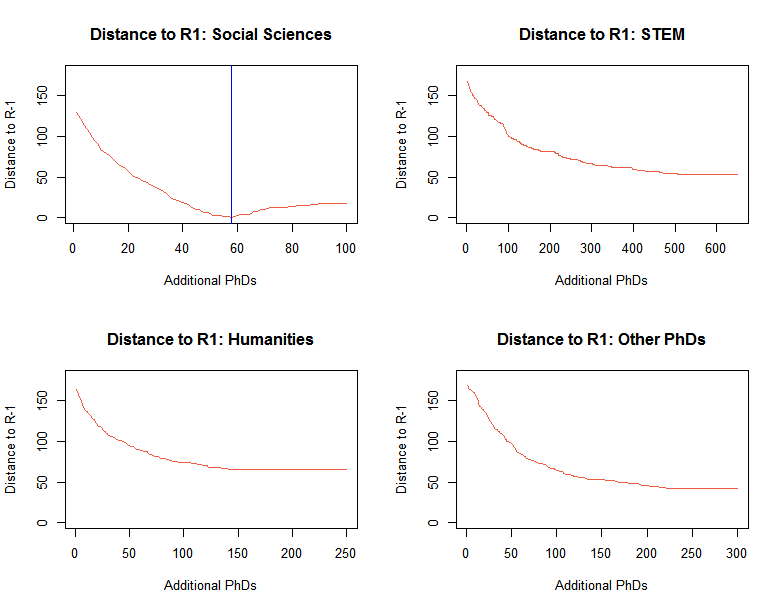
\includegraphics[width=.7\textwidth]{C:/Users/Paul/Documents/Carnegie Classifications/AggDistances}
\captionsetup{font=footnotesize,labelfont=footnotesize}
\caption{\label{fig:agd} Single Variable Movement: Increasing counts of a single type of PhD lead to movement to the right on the plot. However, only a 58 PhD increase in Social Sciences would get Montana State across the R1 border.}

\end{figure}

\subsection{Single Variable Movement: Both Indices}

If increasing awarded doctoral degrees is not enough to move the institution to R1, could the variables that count for both indices work? Indeed, increasing PhDs awarded only moves a given institution to the right or left since those covariates only influence the aggregate index; however, the Stem Expenditures, Non-Stem Expenditures, and Research Staff variables affect both the per-capita and aggregate indices. Thus, increases in either of those three covariates could lead to a given institution moving both up and to the right.  It would seem reasonable, then, that changes in any of the variables used in both indices could be enough to move Montana State across the R1 border. \\
  Reasonable though the theory may sound, the plots in Figure \ref{fig:agb} indicate that neither Stem expenditures, non-Stem expenditures, nor additional research staff can, in and of themselves, move Montana State into the R1 status. Montana State had 75 research staff in 2015; to move up to the top rank the institution would need to add 7223 additional researchers (to break a tie with Harvard, with 7297). Disregarding the absurdity of adding that many researchers, such an increase would still leave Montana State more than 80 units away from R1, a distance that could be obtained by adding fewer than 20 Social Science doctorates.  Moreover, increasing STEM and non-STEM expenditures even by billions of dollars would only lead to modest decreases in the distance from the R1 boundary. \\


  \begin{figure}
    \centering
      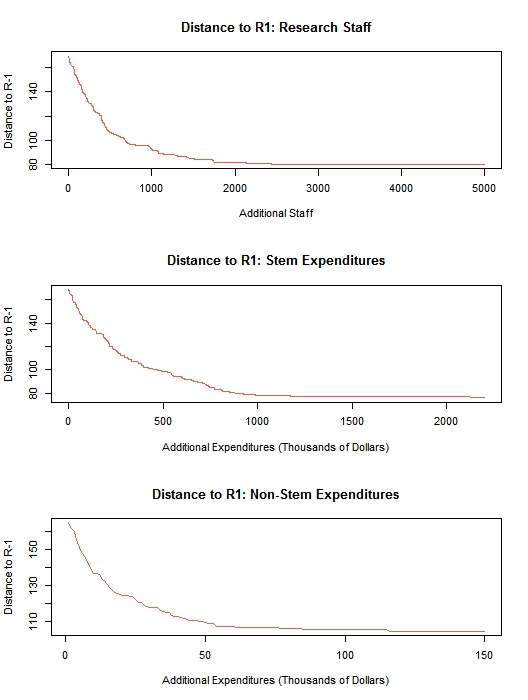
\includegraphics[width=.7\textwidth]{C:/Users/Paul/Documents/Carnegie Classifications/DistR1both}
      \captionsetup{font=footnotesize,labelfont=footnotesize}
   \caption{\label{fig:agb} }{Single Variable Movement: Changes in expenditures and research staff lead to movement in all directions since they are used in both indices. However, increases in any single variable do not lead to large enough movement to get across the R1 threshold.}
   
  \end{figure}


It is worth noting that some single metric changes are more reasonable than others. For instance, while it may be reasonable to consider adding an additional STEM PhD without resulting in changes in the other covariates. However, large increases in STEM expenditures would likely result in more research staff being hired and possibly more PhDs being produced. The above plots only consider movement on single variables without regard to the consequences of those movements.\\  
Ultimately, the narrative that this analysis informs is that in order to move up in the classifications from R2 to R1, decision makers must focus on a multi-dimensional approach. While increases in a single covariate will help move the university up towards the boundary, changes in multiple variables simultaneously will prove much more effective. 


\subsection{Shiny App: Simultaneous Movements}
Movement on multiple dimensions is hard to analyze for several reasons. First, there are eight variables to consider, all of which could increase or decrease in the next update. There are countless combinations of changes in each variable that could hypothetically occur. I created an application using the R package Shiny (Winston 2016) that allows for interactive modeling of changes in the classifications. The application is intended to be used by institutional researchers, administrators, and other stakeholders at Montana State for simulating the classifications under any of those circumstances. \\

The application can be found at the following URL: \texttt{https://paulharmon.shinyapps.io/Carnegie2/}. The end user can adjust Montana State's of PhDs, expenditures, or research staff by moving the slide bars. The application then re-ranks, re-calculates the two PCAs, and plots the new classifications. Small perturbations may change where Montana State falls in the plot, but they do not necessarily change the structure of the classifications; however, large changes in the values for Montana State can actually change the locations of other schools in the ranked PCA, even though their values are held constant for all variables.  This highlights an important feature of the Carnegie Classifications: changes in one school can actually impact the position of other schools. \\

The following plots illustrate a handful of changes that could be made. The first plot illustrates a STEM-heavy change:
\begin{itemize}
\item Increase non-STEM PhD counts by 1 
\item Increase STEM PhDs by 15
\item Double STEM expenditures (Increase by \$104,646)
\item Increase non-STEM expenditures by 5 million dollars
\item Increase research staff by 75
\end{itemize}


  
  Another possible change that could be considered would be to focus solely on non-STEM degrees. Investing in humanities, social sciences, and other non-STEM fields may not be efficient for Montana State given the relative lack of non-STEM infrastructure, but could be considered. Given the dynamics of Montana State, I include small gains to the STEM fields as well. The below scenario involves the following changes:\\
  \begin{itemize}
  \item 10 additional PhDs in all non-STEM categories
  \item 5 additional STEM PhDs
  \item Increase research staff by 25
  \item Increase STEM expenditures by 3 million dollars
  \item Increase non-STEM expenditures by 10 million dollars
  \end{itemize}
  
  Note that this change indicates another key element of the Carnegie Classifications. Well-rounded institutions generally have larger values on both indices than do institutions that specialize only in STEM or non-STEM fields. Compared to the STEM-heavy path, this path seems less arduous; however, there are only a few non-STEM doctoral programs offered at Montana State.   
  

 
 Reducing tenured/tenurable faculty could also help move Montana State towards the boundary; however, it would not be a particularly good long-term solution. The below plot shows where Montana State would be with a reduced tenurable teaching faculty but additional researchers. Reducing faculty may be a way to move towards R1, but it is likely not the best way to do it.  The following scenario considers a 25\% reduction in the size of the tenurable/tenured faculty at Montana State along with modest increases in expenditures, PhDs, and a re-allocation of research faculty. \\
\begin{itemize}
 \item Increase non-STEM PhDs by 1
 \item Increase STEM PhDs by 5
 \item Increase nontenurable research staff by 100
 \item Increase STEM expenditures by 10 million dollars
 \item Increase non-STEM expenditures by 5 million dollars
 \item \textbf{Reduce} tenured/tenurable faculty size by 25\%
\end{itemize}
 

  
  While moving to R1 is the policy goal envisioned by administrators, the specter of moving towards R3 is always a possibility. The following scenario includes small reductions in the number of PhDs produced and research staff combined with wholesale cuts on research expenditures: \\
  \begin{itemize}
  \item Reduce all PhDs by 1 
  \item Reduce non-tenured research staff by 25
  \item Reduce STEM expenditures entirely by 104 million dollars
  \item Reduce non-STEM expenditures by 8 million dollars
    \end{itemize}

  
  The Carnegie Classifications App can be used to model these as well as many other hypothetical scenarios. As a tool for making decisions, it could be used as a starting point for doing economic Cost-Benefit Analysis. Decision-makers could plot out a potential change and then assess the accounting and economic costs of that change in order to determine the lowest-cost methods for potential movements towards R1. Care should be taken when considering these changes; although it may be more mathematically efficient to change one variable, it may not be economically efficient. For instance, adding 10 social science PhDs would likely cost the university more than adding 10 STEM PhDs. Finally, while moving towards R1 classification may not be a bad idea, it is worth remembering that moving towards R3 is just as feasible given the right negative circumstances. 
  
  \pagebreak
\section{Discussion}
  \subsection{Montana State as an R2 Institution}
  Montana State University had previously been classified in the highest tier of "Very High Research Activity" in the 2010 Carnegie Classification update. However, it may not have been well-classified. Most R1 schools produce more doctoral degrees of each type than Montana State; moreover, the typical R1 institutions spend more money on research expenditures in STEM and non-STEM fields than did Montana State.  It is worth recalling that the Carnegie Classifications are not intended to measure quality of educational experience; rather, they are used to identify similar institutions to a given school. In this case, Montana State's research output, size, and expenditures are more similar to North Dakota State University than to, for instance, the University of Michigan; the Carnegie Classifications reflect this. 
  
  
  \subsection{Moving Up: How Hard Would It Be?}
  There is no single way to move from R2 to R1, nor is there a single way to move down to the R3 category Both are possible for Montana State to achieve under the right set of circumstances. While breaking ties can help lead to large movements in the variables, this is likely more important for the Aggregate Index because the PhD counts are more likely to be tied. Montana State could improve from rank 1 to rank 61 in the Social Sciences PhD variable by adding just a single doctorate in the social sciences; this may actually occur with the addition of a Psychology PhD program in 2015.\\ 
  Although Montana State is close to the R1 category, getting across the border would necessitate fairly significant gains in PhDs produced across all four categories and research staff size as well as large increases in STEM and non-STEM expenditures.  The research staff and PhD counts are likely feasible; Montana State's growing infrastructure and faculty allow for increases in those variables that ought to be enough to at least move MSU towards the border. However, without nearly doubling non-STEM expenditures and adding STEM expenditures in the tens of millions of dollars, changes in the underlying variables simply are not enough to get MSU to R1. 
  
  \subsection{Snapshots vs. Averages}
  The data are collected via a snapshot over the course of a year. While expenditures and research staff may stay relatively constant over a period of a few years, counts of PhDs may be relatively variable. Given that uncertain nature of doctoral programs, it is difficult to predict exactly how many PhD students may graduate in a given year (at least compared to undergraduates or master's students). Year-to-year variation in the number of PhDs produced may drive some variability in the classifications. An interesting analysis - one that would require a great deal more data are available in the Carnegie Classifications update - would be to examine a five-year average of all the variables at each institution and compare them to the snapshot-driven analysis performed by the Indiana University Center on Postsecondary Research. 
  
  
  \subsection{Limitations of Static Analysis}
This analysis considers changes at Montana State, holding the values at other institutions constant. Certainly, the assumption that other institutions will stay static over the next five years is unrealistic; however, we cannot predict with a high degree of certainty how other institutions will change before the next update.This analysis should be treated in a manner similar to that of a linear regression problem with multiple covariates; in such a situation, parameters are estimated under the assumption that the others are held constant. In this instance, the same methodology can be applied; these small perturbations are made under the assumption that the data for other institutions are not simultaneously changing. \\

One way for policy makers at Montana State to attempt to circumvent this problem would be to think less about the borders between the groups themselves and rather focus on moving to a point in the center of the R1 designation. The delineations between each group are the least predictable and most likely to change aspect of the classifications. Instead of trying to determine the most efficient way to get to the border, I would suggest that policy makers make getting to a central position in the R1 cluster a goal.  

\subsection{Final Thoughts}
The Carnegie Classifications are useful for institutional research; however, their efficacy as metrics of institutional quality is highly questionable. R1 schools are not intended to be thought of as better than R2 schools; however, some campus administrators, faculty, and media have used them in this way. The delineations between each group are highly subjective; moreover, the nature of the dimension reduction used to create both indices leaves room for some debate. The Carnegie Classifications would contain more information about the underlying covariates if more than a single Principal Component were used in each index.  Finally, the nature of the self-reported snapshot data used in this analysis leads to the possibility of miscalculation due to either clerical errors, different definitions of variables at different schools, or other problems. The data may not be entirely consistent across institutions.  Given all this, the Carnegie Classifications should be taken with a grain of salt. They are useful tools for identifying similar institutions; however, prioritizing one status over another is not an appropriate policy goal for any institution of higher education, including Montana State University. 

\end{doublespace}
\pagebreak
\begin{thebibliography}{9}
	
\bibitem{ties}
Becker, R. A., Chambers, J. M. and Wilks, A. R. (1988) \textit{The New S Language}. Wadsworth and Brooks/Cole.
	
\bibitem{PersonalCommmunication}
Borden, V. (March 2017). \textit{Personal Communication}.


\bibitem{EandH}
Everitt, B., and Hothorn, T. (2011). \textit{An introduction to applied multivariate analysis with R}. Berlin: Springer.
\bibitem{Elements}
Friedman, J., Hastie, T., and Tibshirani, R. (2009). \textit{The Elements of Statistical Learning: Data Mining, Inference, and Prediction} (2nd ed.). Springer.
\bibitem{beanplot}
Kampstra, P. (2008). \textit{Beanplot\: A Boxplot Alternative for Visual Comparison of Distributions}. Journal of
Statistical Software, Code Snippets 28(1). 1-9. \texttt{http://www.jstatsoft.org/v28/c01/}.
\bibitem{mcclintick}
McClintick, W. (2016). \textit{Carnegie Sensitivity Analysis: Moving from R2 to R1}. Poster Presentation at Rocky Mountain Association of Institutional Research Conference.

\bibitem{Grizz} 
University of Montana. (2017). \textit{UM Strategic Mission 1.0\: Creating Change Together}. Missoula, MT. \textit{http://www.umt.edu/strategy/strategic-vision/UM\_Strategic\_Vision\_1\_0.pdf}

\bibitem{West}
West, M. (2003). Bayesian Factor Regression Models in the “Large p, Small n” Paradigm. \textit{Bayesian Statistics}, 723-732.




\end{thebibliography}

\end{document}